\documentclass[12pt]{article}
\usepackage[margin=2.5cm]{geometry}
\usepackage{enumerate}
\usepackage{amsfonts}
\usepackage{amsmath}
\usepackage{fancyhdr}
\usepackage{amsmath}
\usepackage{amssymb}
\usepackage{amsthm}
\usepackage{mdframed}
\usepackage{graphicx}
\usepackage{subcaption}
\usepackage{adjustbox}
\usepackage{listings}
\usepackage{xcolor}
\usepackage{booktabs}
\usepackage[utf]{kotex}
\usepackage{hyperref}

\definecolor{codegreen}{rgb}{0,0.6,0}
\definecolor{codegray}{rgb}{0.5,0.5,0.5}
\definecolor{codepurple}{rgb}{0.58,0,0.82}
\definecolor{backcolour}{rgb}{0.95,0.95,0.92}

\lstdefinestyle{mystyle}{
    backgroundcolor=\color{backcolour},
    commentstyle=\color{codegreen},
    keywordstyle=\color{magenta},
    numberstyle=\tiny\color{codegray},
    stringstyle=\color{codepurple},
    basicstyle=\ttfamily\footnotesize,
    breakatwhitespace=false,
    breaklines=true,
    captionpos=b,
    keepspaces=true,
    numbers=left,
    numbersep=5pt,
    showspaces=false,
    showstringspaces=false,
    showtabs=false,
    tabsize=1
}

\lstset{style=mystyle}

\pagestyle{fancy}
\renewcommand{\headrulewidth}{0.4pt}
\lhead{CSC 209}
\rhead{Review 6 Solution}

\begin{document}
\title{CSC 209 Review 6 Solution}
\maketitle

\bigskip

\section{Exercises}

\begin{enumerate}[1.]
    \item

    I need to write which of the supplied function calls don't work and explain why.

    \bigskip

    \begin{itemize}
        \item \texttt{b)} String format in \texttt{printf} expects character constant, but string literal is used
        \item \texttt{c)} String format in \texttt{printf} expects string but character constrant is used
        \item \texttt{e)} The first argument in \texttt{printf} expects pointer but character constrant (an integer) is used isntead
        \item \texttt{h)} The first argument in \texttt{putchar} expects a character, but string literal (a pointer to character) is used
        \item \texttt{i)} The first argument in \texttt{puts} expects a pointer to character, but character constant (an integer) is used
    \end{itemize}

    \underline{\textbf{Notes}}

    \begin{itemize}
        \item \textbf{putchar}

        \begin{itemize}
            \item \textbf{Syntax:} \texttt{int putchar(int char)}
            \item Writes a character (an unsigned char) specified by the argument char to stdout.
            \item Does not append a new line to the output
            \item Is similar to printf but for character
        \end{itemize}

        \item \textbf{puts}

        \begin{itemize}
            \item \textbf{Syntax:} \texttt{int puts(const char *str)}
            \item Writes a string to stdout up to but not including the null character
            \item Appends a newline character to the output.
            \item Is similar to printf but for string
        \end{itemize}

        \item \textbf{Character Constant}

        \begin{itemize}
            \item \textbf{Syntax:} \texttt{' ... '}
            \item Is represented by an \underline{integer}
        \end{itemize}

        \item \textbf{String Literal}
        \begin{itemize}
            \item \textbf{Syntax:} \texttt{" ... "}
            \item Has a sequence of characters inside
            \item Ends with \texttt{$\backslash$0}
            \item Is represented by a \underline{pointer}

            \bigskip

            \underline{\textbf{Example}}

            \bigskip

            "When you come to a fork in the road, take it"
        \end{itemize}

        \item \textbf{Escape Squences in String Literal}

        \begin{itemize}
            \item A common example is `\texttt{$\backslash$n}'

            \begin{itemize}
                \item causes the cursor to advance to the next line
            \end{itemize}
        \end{itemize}
    \end{itemize}

    \item

    First, I need to write which of the provided function calls are legal, and write the output
    produced

    \bigskip

    The solution to the first part is:

    \begin{itemize}
        \item \texttt{b)} [output: a]
        \item \texttt{c)} [output: abc]
    \end{itemize}

    \bigskip

    Second, I need to write which of the following function calls are illegal, and explain why.

    \bigskip

    The solution to the second part is:

    \begin{itemize}
        \item \texttt{a)} \texttt{purchar} expects a character constant (an integer) but a value of type pointer to \texttt{char} is used
        \item \texttt{d)} \texttt{puts} expects a variable of type pointer to \texttt{char}, but a variable of type pointer to \texttt{char} is used
    \end{itemize}

    \item

    I need to write the values of \texttt{i}, \texttt{j}, \texttt{k} in the function

    \bigskip

    \texttt{scanf("\%d\%s\%d", \&i, s, \&j)}

    \bigskip

    if the user enters \texttt{12abc34 56def78}.

    \bigskip

    The solution to this problem is:

    \begin{itemize}
        \item \texttt{i} - \texttt{12}
        \item \texttt{j} - \texttt{abc34 }
        \item \texttt{k} - \texttt{56}
    \end{itemize}

    \item

    I need to modify the following \texttt{read\_line} function in the following ways:

    \begin{center}
    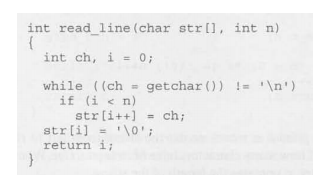
\includegraphics[width=0.7\linewidth]{images/review_6_solution_1.png}
    \end{center}

    \begin{enumerate}[a)]
        \item Have it skip white space beore beginning to store input characters
        \item Have it stop reading at the first white-space character
        \item Have it stop reading at the first new-line character, then store the new-line character in the string
        \item Have it leave behind characters that it doesn't have room to store
    \end{enumerate}

    \bigskip

    The solution to this problem is:

    \begin{enumerate}[a)]
        \item

\begin{lstlisting}[language=c]
    #include <ctype.h>
    #include <stdbool.h>

    ...

    int read_line(char str[], int n)
    {
        int ch, i = 0;
        bool non_space_char_exists = false;

        while ((ch = getchar()) != '\n')
            if (isspace(ch) && non_space_char_exists){
                continue;
            }

            if (i < n)
                str[i++] = ch;
                non_space_char_exists = true;
        str[i] = '\0';
        return i;
    }
\end{lstlisting}

        \item

\begin{lstlisting}[language=c]
    #include <ctype.h>

    ...

    int read_line(char str[], int n)
    {
        int ch, i = 0;

        while ((ch = getchar()) != '\n')
            if (isspace(ch)){
                break;
            }

            if (i < n)
                str[i++] = ch;
        str[i] = '\0';
        return i;
    }
\end{lstlisting}

        \item

\begin{lstlisting}[language=c]
    #include <ctype.h>

    ...

    int read_line(char str[], int n)
    {
        int ch, i = 0;

        while ((ch = getchar()) != '\n')
            if (ch == '\n'){
                break;
            }

            if (i < n)
                str[i++] = ch;

        str[i] = '\n';
        str[i+1] = '\0';
        return i;
    }
\end{lstlisting}

        \item

\begin{lstlisting}[language=c]
    #include <ctype.h>

    ...

    int read_line(char str[], int n)
    {
        int ch, i = 0;
        int n = strlen(str) + 1;

        do {
            ch = getchar();

            if (!ch) {
                break;
            }

            str[i++] = ch;

        } while (i < (n - 1));

        str[i] = '\0';
        return i;
    }
\end{lstlisting}


    \end{enumerate}

    \bigskip

    \begin{mdframed}
    \underline{\textbf{Correct Solution}}

    \bigskip

    \begin{itemize}

        \item \texttt{c)}

\begin{lstlisting}[language=c]
    #include <ctype.h>

    ...

    int read_line(char str[], int n)
    {
        int ch, i = 0;

        do {
            ch = getchar()

            if (ch == '\n'){
                break;
            }

            if (i < n)
                str[i++] = ch;

        } while (ch !== '\n');

        str[i] = '\0';
        return i;
    }
\end{lstlisting}

        \item \texttt{d)}

\begin{lstlisting}[language=c]
    #include <ctype.h>

    ...

    int read_line(char str[], int n)
    {
        int ch, i = 0;
        int n = strlen(str) + 1;

        do {
            ch = getchar();

            if (ch == '\n') {
                break;
            }

            str[i++] = ch;

        } while (i < (n - 1));

        str[i] = '\0';
        return i;
    }
\end{lstlisting}


    \end{itemize}


    \end{mdframed}

    \bigskip

    \underline{\textbf{Notes}}

    \begin{itemize}
        \item Learned that \texttt{getchar()} always ends with \texttt{$\backslash$n}
    \end{itemize}

    \item

    \begin{enumerate}[a)]
        \item

        I need to write a function named \texttt{capitalize} that capitalizes all
        letters in its argument.

        \bigskip

        The requirement for this function is:

        \bigskip

        \begin{itemize}
            \item Array subscripting must be used to access each character in string
        \end{itemize}

        \bigskip

        The solution to this problem is:

        \bigskip

\begin{lstlisting}[language=c]
    #include <ctype.h> // toupper

    void capitalize(char *s)
    {

        for (int i = 0; s[i] != '\0'; i++) {
            s[i] = toupper(s[i]);
        }
    }
\end{lstlisting}

        \bigskip

        \underline{\textbf{Notes}}

        \begin{itemize}
            \item \textbf{Accessing the Characters in a String}

            \begin{enumerate}[1.]
                \item Using array subscripting

                \bigskip

                \underline{\textbf{Example}}

                \bigskip

                \begin{center}
                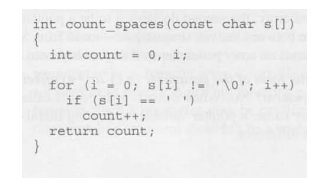
\includegraphics[width=0.7\linewidth]{images/review_6_solution_2.png}
                \end{center}

                \bigskip

                \item Using pointer

                \bigskip

                \underline{\textbf{Example}}

                \bigskip

                \begin{center}
                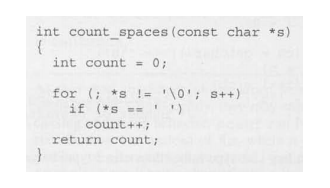
\includegraphics[width=0.7\linewidth]{images/review_6_solution_3.png}
                \end{center}

                \bigskip

            \end{enumerate}
        \end{itemize}

        \item

        I need to write a function named \texttt{capitalize} that capitalizes all
        letters in its argument.

        \bigskip

        The requirement for this function is:

        \bigskip

        \begin{itemize}
            \item pointer must be used to access each character in string
        \end{itemize}

        \bigskip

        The solution to this problem is:

        \bigskip

\begin{lstlisting}[language=c]
    #include <ctype.h> // toupper

    void capitalize(char *s)
    {
        char *p = s;
        while (*p != '\0') {
            *p = toupper(*p);
            p++;
        }
    }
\end{lstlisting}


    \end{enumerate}

\end{enumerate}


\end{document}